%%% Fiktivní kapitola s ukázkami sazby

\chapter{Návrh řešení}

V této kapitole je popsán návrh technického řešení uvedených problémů.

\section{Úvod}

Běh celé aplikace bude rozdělen do dvou částí.

\begin{itemize}
	\item Stahování a ukládání real-time dat o polohách vozidel do datového skladu, které budou doplněny o odhat zpoždění pro okamžité zveřejnění v uživatelské aplikaci.

	\item Modelování profilů jízd jednotlivých úseků. Tyto modely budou pak dále sloužit k odhadování zpoždění v budoucnu.  Výpočet modelů bude prováděn jednou za delší časový úsek (nejlépe jednou za den).
\end{itemize}

Protože obě části jsou na sobě závislé v iniciálním běhu bude prováděna první část sběru dat bez odhadu zpoždění, nebo pomocí již existujícího triviálního lineárního odhadu.

\bigbreak

Schéma návrhu celé aplikace a komunikační mapa jednotlivých komponent je ilusrtována na diagramu \ref{fig:design_diagram}.

\begin{figure}
	\centering
  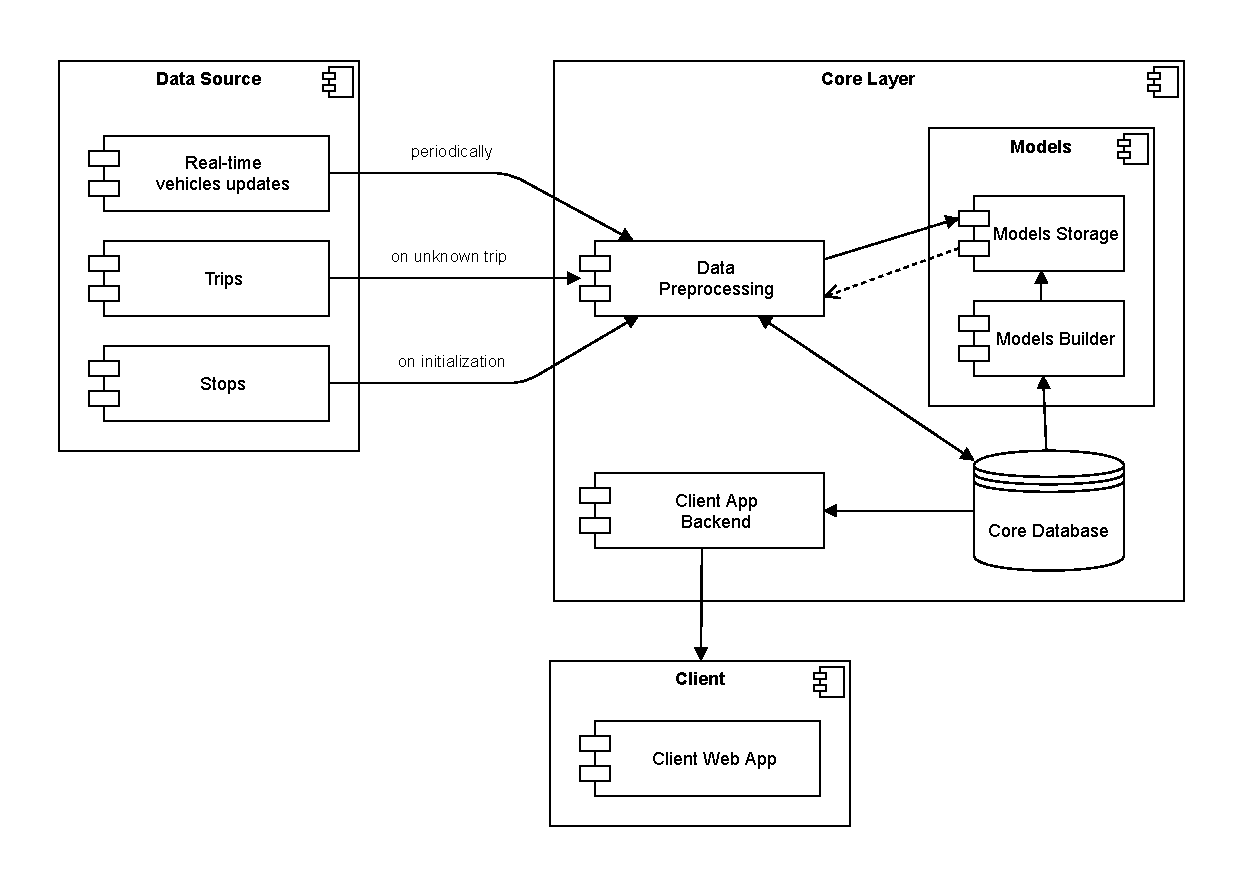
\includegraphics[width=140]{../img/design_diagram}
  \caption{UML diagram návrhu aplikace}
  \label{fig:design_diagram}
\end{figure}

\subsection{Funkční a kvalitativní požadavky}

Nejprve specifikujme požadavky systému, na kterém se pak bude zakládat
konkrétní návrh řešení backendu celé aplikace (bez vizualizace).

\subsubsection{Funkční požadavky}

\begin{itemize}
	\item
Popsaný odhad změny zpoždění na trase mezi dvěma referenčními body je nutné počítat v co nejkratším čase tak, aby cestující byli dobře informování o stavu jejich spoje a mohli tyto informace využít např. při dobíhání spoje. A proto je potřeba zpracovávat data okamžitě po jejich vydání, spočítat odhad zpoždění a vystavit tato data veřejně. Vzhledem k tomu, že tato data velmi rychle zastarávají je nutné provádět tento proces co možná nejrychleji\footnote{Průměrná doba jízdy spoje mezi zastávkami je cca 5 min. Rozložení počtu úseků mezi zastávekami k délce jízdy mezi nimi je závislé a podobné rozložení vůči vzdálenosti ilustrované na grafu\ref{fig:stop_distances_result}.}.

\item

Data o polohách vozidel VHD v Datové platfomě jsou aktualizována nejpozději každých 20 sekund, více v kapitole \ref{chapter:analyza_zdroje}. Tedy pro minimalizaci rychlosti zastarávání dat a získání všech existujících vzorků dat o polohách je nutné data stahovat alesponˇ každých 20 sekund.

\item

Odhad zpoždění se bude provádět na základě historických dat z posledních vyšších jednotek dnů\footnote{Pro demonstrativní účely této práce jsou využívány historická data pouze ze 4 dnů (2 pracovní a 2 víkendové).}. Tím se sníží dopad mimořádné události na předpovědní model, která může na trase vzniknout. Zárovenˇ by však neměla být započítávána data starší několik týdnů, protože dopravní situace se mění v závislosti na ročním období nebo také pokud je na trase delší omezení dopravy je požadováno, aby se takové omezení projevilo co možná nejdříve. Navíc se bude rozlišovat mezi daty z pracovních dnů a nepracovních dnů, to protože samotné jízdní řády se mohou lišit (doba jízdy mezi mezastávkama) a také se do velké míry liší hustota dopravy, která ma velký vliv na profil jízdy. TODO do navrhy na zlepseni: Pro zpřesnění výsledků by bylo lepsi respektovat svatky, kazdy den v tydnu zvlast atp.

\item

Zpracování historických dat bude probíhat vždy po delší době, nejlépe jednou za den. To umožní provádět náročnější výpočty, které by za normálního provozu neúměrně přetížily systém. Navíc vzhledem k povaze cíle práce ani není žádoucí zpracování historických dat provádět častěji než jednou denně, protože se nepokoušíme okamžitě reagovat na změnu dopravní situace.

\item

Uložená historická data budou struktorovaná tak, aby nad nimi šly provádět statistické výpočty minimálně o frekvencích spojů, vzdálenostech tras, zpoždění spojů.
\end{itemize}

\subsubsection{Kvalitativní požadavky}

\begin{itemize}

	\item
	Řešení bude schopno při jedné aktualizaci zpracovat alesponˇ 1000\footnote{20. 2. 2020 mezi 7:00 a 7:10 bylo na trase přes 600 vozidel} vzorků poloh vozidel, kde 10 \% vzorků může být o dosut neznámých jízdách. V tomto případě je potřeba stáhnout jízdní řád konkrátní jízdy a její jízdní profil, což navíc dotaz na zdroj dat.

	\item
	Vypočítané modely profilů jízd budou dávat odhat zpoždění lepší, než je lineární odhad. To znamená, že zpoždění vypočítaná pro každý přijatý vzorek polohy vozidla mezi dvěma referenčními body na trase bude mít menší rozptyl než lineární odhad zpoždění.

\end{itemize}


\section{Zpracování vstupních dat}

Struktura uložení dat se zakládá na struktuře zdrojových dat popsaných v kapitole \ref{section:analyza_zdroje} Analýza zdroje dat.

\bigbreak

Na datové platformě jsou real-time data o vozidlech dostupná do historie řádově jednotek minut, což je naprosto nedostatečné pro jakékoliv pozdější využití v ránci této práce. Především pro počítání statistik a modelování profilů jízd nad daty je potřeba zřídit lokální databázi, která bude držet historická data tak, jak byla obdržena od zdroje. Navíc data jsou poskytována ve formátu \gls{json}, který svou povahou není zrovna úsporný co se do velikosti souboru týče. Proto je vhodné zvolit ukládání dat v jiném formátu.

\subsection{Databáze}

Za tímto účelem tato práce využívá relační databázi obsluhovanou dotazovacím jazykem \gls{sql}. Struktura databáze je vyobrazena na EER diagramu \ref{obr:EER}\footnote{SQL dotazy na sestavení celé databaze jsou definovány v příloze database.sql. Pro testovací, debugovací a demonstrační účely slouží navíc i jiné databáze, které jsou struktorou totožné jako produkční databáze.}. Tato databáze se skládá z 5 tabulek. Jsou jimi:


\begin{figure}[p]\centering
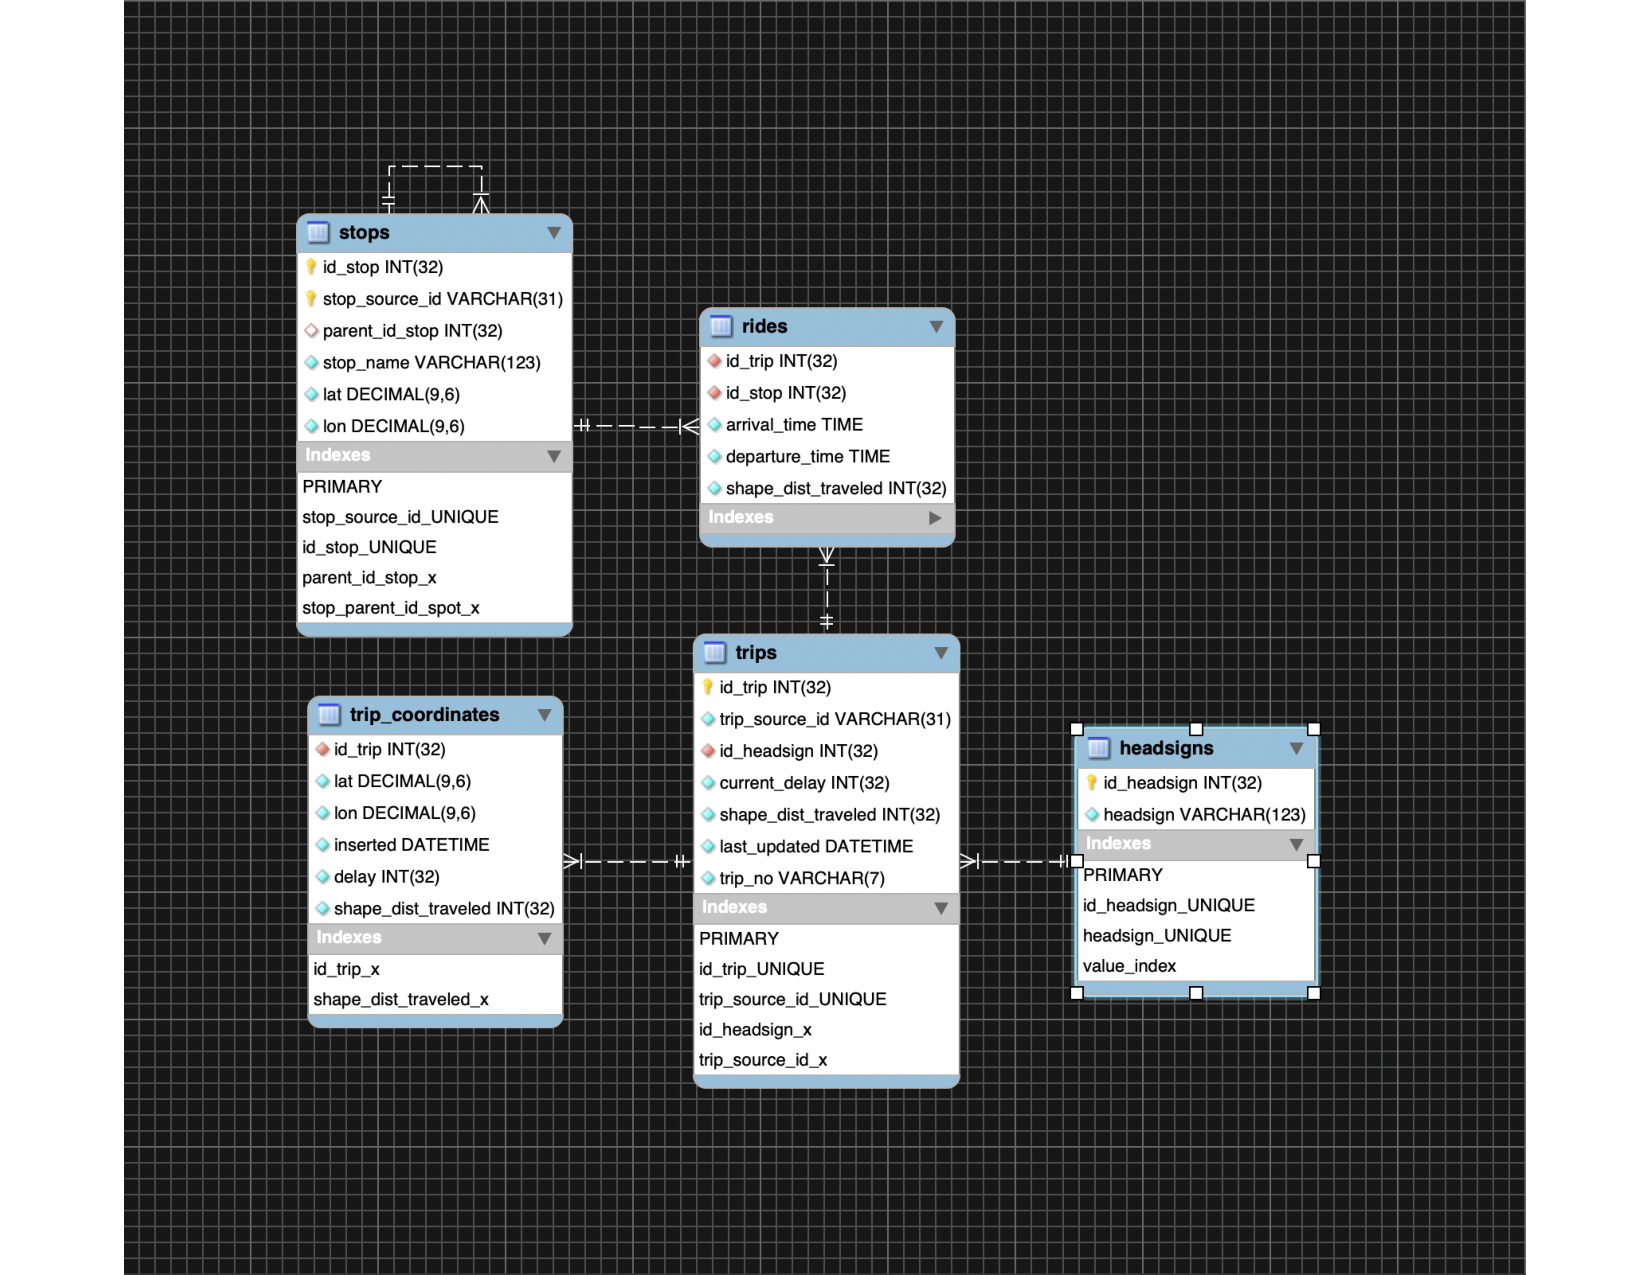
\includegraphics[width=140mm]{../img/eer_database}
% Příponu není potřeba explicitně uvádět, pdflatex automaticky hledá pdf.
% Rozměry také není nutné uvádět.
\caption{EER diagram databáze.}
\label{obr:EER}

\end{figure}

\begin{itemize}
	\item \verb-trips- všechny objevené jízdy

		\begin{itemize}
			\item \verb-id_trip- unikátní identifikátor používaný v databázi

			\item \verb-trip_source_id- identifikátor tripu převzatý ze zdroje dat

			\item \verb-id_headsign- identifikátor nápisu pro daný trip

			\item \verb-current_delay- aktuální zpoždění tripu

			\item \verb-shape_dist_traveled- aktuální vzdálenost ujetá od výchozí stanice

			\item \verb-last_updated- čas poslední aktualizace, převzatý ze zdroje dat

			\item \verb-trip_no- číslo dané linky
		\end{itemize}

	\item \verb-headsigns- nápisy nad vozidlem, cílová stanice

		\begin{itemize}
			\item \verb-id_headsign- unikátní identifikátor nápisu

			\item \verb-headsign- text nápisu
		\end{itemize}

	\item \verb-trip_coordinates- všechna historická real-time data

		\begin{itemize}
			\item \verb-id_trip- identifikátor tripu, ke kterému se záznam váže

			\item \verb-lat- zeměpisná šířka polohy vozidla

			\item \verb-lon- zeměpisná délka polohy vozidla

			\item \verb-inserted- čas vložení záznamu

			\item \verb-delay- zpoždění zachycené v poslední projeté stanici před pořízením záznamu

			\item \verb-shape_dist_traveled- vzdálenost ujetá od výchozí stanice tripu

		\end{itemize}

	\item \verb-stops- všechny zastávky

		\begin{itemize}
			\item \verb-id_stop- unikátní identifikátor zastávky

			\item \verb-trip_source_id- identifikátor zastávky převzatý ze zdroje dat

			\item \verb-parent_id_stop- identifikátor rodičovské zastávky, pokud existuje

			\item \verb-stop_name- název zastávky

			\item \verb-lat- zeměpisná šířka polohy zastávky

			\item \verb-lon- zeměpisná délka polohy zastávky

		\end{itemize}

	\item \verb-rides- trasa každého tripu, seznam zastávek s časy odjezdů a příjezd tvořící jízdní řád

	\begin{itemize}
		\item \verb-id_stop- identifikátor tripu

		\item \verb-id_stop- identifikátor zastávky

		\item \verb-arrival_time- čas příjezdu tripu do zastávky

		\item \verb-departure_time- časodjezduu tripu ze zastávky

		\item \verb-shape_dist_traveled- vzdálenost zastávky od výchozí zastávky tripu

	\end{itemize}

\end{itemize}

Atributy se jménem *source\_id jsou pravděpodobně unikátní identifikátor entity ve zdroji dat, nicméně z dokumentace zdroje to nevyplývá. Také je tento indenfikátor ukládán jako textový řetězec, ačkoli je tvořen pouze číslicemi a podtržítky, není nikde zaručeno, že jej lze jednoduše převést na číselný ko'd. Takže pro lepší výkon databáze je použito automaticky generované id typu \gls{int}.

\bigbreak

Každá tabulka má několik indexů, které zlepšují výkon databáze při vkládání a hledání dat. Obvzláště pokud je atribut označen jako unikátní, kde se při každém vložení ověřuje unikátnost.

\bigbreak

Databáza je nastavená tak, aby umožňovala získat všechny potřebné informace o vozidlech, ale hlavně přístup k historickým real-time datům a to separovaně pro dvojci refenčních bodů.

\subsection{Plnění databáze}

Tato databáze bude plněna skriptem, jehož bude naprogramován taky, aby vždy stáhl aktuální obraz dopravní situace a tato data uložil do dotabáze. Toto stahování z datové platformy probíhá podle násldujícího algoritmu.

\bigbreak

Algoritmus:
\begin{code}[frame=none]
načti všechny dostupné zastávky
dokud skrip běží
  načti aktuální polohy vozidel
  pro každé nalezené vozidlo
  pokud jízda vozidla je známá
    aktualizuj data o jízdě
  jinak
    stáhni informace o jízdě
    zpracuj a vlož jízdu do databáze
\end{code}

\bigbreak

Protože všechny infomace ukládané do databáze jsou důležité pro hlavní cíl této práce, tak pokud se vyskytne jízda, který neobsahuje některou z požadovaných infomarcí je pak automaticky zahozena. To je řešeno pomocí databázových transakcí tak, aby stav databáze byl vždy konzistentní. Transakce v obecném smyslu fungují tak, že můžeme měnit data v databázi (i více zázanamů) a tyto změny se zapíší do samotné databáze až po potvrzení, že všechny změny byly provedeny správně, pokud během provádění změn nastane chyba, můžeme v jakékoli fázi provádění změn všechny dosud proveedné změny zahodit a vrátit se do původního stavu databáze před započetím transakce.  Tedy pokud nejsou poskytnuta data ve formátu, který skript akceptuje, nebo nějaké povinné atributy chybí. Vložení celé jízdy nebude provedeno.

\bigbreak

Nejčastěji chybějící atribut je zpoždění v poslední zastávce, toto je nutné vědět pro počítání zpoždění mezi refenrečními body (zastávkami). Absence této informace může být způsobena tím, že vozidlo vůbec nevysílá data potřebnák k jejím dopočtení, pak nemá smysl jej do databáze zahrnovat. Nebo vozidlo už vysílá, ale ještě nezahájilo jízdu, tedy nemá žádnou poslední projetou zastávku, v takovém případe budou data ignorována až do doby příchodu první relevantní informace.

\bigbreak

Mimo popsanou databázi se do určeného adresáře ukládají trasy jednotlivých jízd, která jsou ve fromátu \gls{geojson} jako lomená čára definována souřadnicemi. Navíc data o trasách jsou používána pouze pro vizualizaci a jsou přijímány vizualizačním nástrojem ve formátu \gls{geojson}, tedy tyto data není nutné vůbec transformovat a není nutné je držet v hlavní databázi.

\bigbreak

 Stejně tak i aktuální polohy vozidel jsou mimo databázi zapisovány do souboru, který je určen a formátován pro čtení webovou aplikací. Aktualizace tohoto souboru je provedena přednostně, ihned po načtení real-timových dat. Tím se zabrání nechtěnému čekaní na aktualizaci celé databáze, která může trvat jednotky sekund.


\section{Algoritmus odhadu zpoždění}



\section{Vizualizace dat}

\subsection{Funkční požadavky}

\begin{itemize}
	\item

	\item Aplikace vykreslí interaktivní mapu Prahy a širšího okolí, kterou bude možné posouvat či zoomovat. V této mapě budou zobrazeny vozidla na aktuálních pozicích a budou se automaticky posouvat po mapě, tak jak se pohybují ve skutečnosti.

	\item Po kliknutí na vozidlo se zobrazí jeho celá trasa včetně zastávek a jeho dopočítaného zpoždění.

	\item Po kliknutí na zastávku se zobrazí seznam spojů, které budou projíždět vybranou zastávkou a jejich trasy se vykreslí do mapy.

	\item Celá aplikace bude postavena na principu server -- client. Tedy serverová strana se postará o přístup k otevřeným datům o vozidlech a jejich uložení a také obsluhu požadavků klienta. Klientská část bude webová stránka poskytující služby popsané výše. Měla by být schopná zobrazit řádově tisíce vozidel.
\end{itemize}

\subsubsection{Nefunkční požadavky}

\begin{itemize}
	\item Serverová část bude napsaná v jazyce Python 3.

	\item Webová část bude napsaná pomocí jazyků pro webové technologie, převážně v JavaScriptu.

	\item Pro vykleslení mapy bude využita služba Mapbox.

	\item Ukládání dat na serverové straně bude řešeno MySQL databází.

	\item Pro algoritmus odhadu zpoždění na zákldě historických dat budou využity různé knihovny pro jazyk Python 3. Zejména pak scikit-learn a alphashape.

\end{itemize}

\subsubsection{Proces běhu aplikace}

Jak je již zmíněno aplikace bude využívat historická data, tedy bude nutné nechat aplikaci tato data nějakou dobu sbírat. Pro efektivní odhady by bylo vhodné mít uložené historické polohy vozidel alespoň z uplynulých několika týdnů.

\bigbreak

Avšak již v průběhu sběru dat může aplikace poskytovat základní službu a to vizualizování vozidel v mapě.

\subsection{Poskytovatelé mapových podkladů}

K takovému účelu nejlépe poslouží vykreslení aktuálních poloh vozidel do mapy, kde se po vyžádání uživatelem tyto data zobrazí.

\bigbreak

Za účelem vytvoření dostatečně přívětivé uživatelské aplikace je nezbytné využít některého z poskytovatelů mapových podkladů a zanést do něj získané informace.

\bigbreak

Jedním z těchto poskytovatelů je společnost Google, která má propracované mapové podklady a prostřednictvím služby Google Maps poskytuje pro tuto práci požadovanou službu. Další platformou je Mapbox, který poskytuje velmi podobné služby jako Google Maps. Nicméně narozdíl od Googlu využívá jako mapový podklad \gls{osm} {otevřená geografické data}. Protože smyslem práce je v co největší míře využít otevřená data je žádoucí využít právě Mapbox.

\bigbreak

TODO dokumentace mapbox, zeptat se jestli je to vubec nutne rozebirat
